\documentclass[12pt]{article}
\usepackage[margin=2cm]{geometry}
\usepackage{tikz}
\usetikzlibrary{patterns, calc, arrows.meta, shapes.geometric, positioning}
\usepackage{enumitem}
\usepackage{amssymb}

\pagestyle{empty}

\tikzset{
    celda/.style={draw, minimum size=1.5cm, inner sep=0pt, line width=0.5pt},
    sombreado/.style={fill=black!80},
    opbox/.style={draw, minimum size=1.1cm, inner sep=0pt, line width=0.4pt},
}

\begin{document}

\begin{center}
{\Large\bfseries HABILIDAD MATEM\'ATICA}\\[3pt]
{\normalsize Examen diagn\'ostico --- 16 preguntas}
\end{center}

\bigskip

%%% ============================================================
%%% BLOQUE 1: SUCESIONES NUMÉRICAS (Preguntas 1--4)
%%% ============================================================

\noindent\textbf{1.}\quad ¿Qué números continúan en la siguiente sucesión?

\medskip
\centerline{\textbf{60, 17, 48, 14, 36, 11, \underline{\quad}, \underline{\quad}, \ldots}}
\medskip

\begin{enumerate}[label=\Alph*), nosep, leftmargin=2cm]
\item 24, 8
\item 28, 9
\item 24, 9
\item 24, 7
\end{enumerate}

%% Respuesta: A
%% Lógica: Dos sucesiones intercaladas.
%% Pares: 60, 48, 36, 24 (resta 12)
%% Impares: 17, 14, 11, 8 (resta 3)

\bigskip

\noindent\textbf{2.}\quad El número que sigue en la sucesión 
\textbf{2, 5, 15, 18, 54, 57, \underline{\quad}} es

\medskip
\begin{enumerate}[label=\Alph*), nosep, leftmargin=2cm]
\item 171
\item 60
\item 114
\item 174
\end{enumerate}

%% Respuesta: A
%% Lógica: Patrón alternante: ×3, +3, ×3, +3, ×3, +3
%% 2 ×3=6? No... let me recalculate
%% 2, +3=5, ×3=15, +3=18, ×3=54, +3=57, ×3=171
%% Sí: +3, ×3, +3, ×3, +3, ×3 → 171

\bigskip

\noindent\textbf{3.}\quad Encuentra los términos que continúan la sucesión.

\medskip
\centerline{\textbf{5, 8, 10, 16, 20, 32, \underline{\quad}, \underline{\quad}, \ldots}}
\medskip

\begin{enumerate}[label=\Alph*), nosep, leftmargin=2cm]
\item 40, 64
\item 40, 48
\item 44, 64
\item 36, 64
\end{enumerate}

%% Respuesta: A
%% Lógica: Dos sucesiones intercaladas.
%% Posiciones impares: 5, 10, 20, 40 (×2 cada vez)
%% Posiciones pares: 8, 16, 32, 64 (×2 cada vez)

\bigskip

\noindent\textbf{4.}\quad ¿Qué números completan la secuencia de la cadena?

\begin{center}
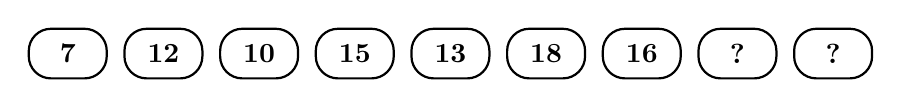
\begin{tikzpicture}[scale=0.9]
% Cadena de óvalos eslabonados
\foreach \i/\val in {0/7, 1/12, 2/10, 3/15, 4/13, 5/18, 6/16} {
    \draw[line width=0.8pt, rounded corners=8pt] (\i*1.35-0.55, -0.35) rectangle (\i*1.35+0.55, 0.35);
    \node at (\i*1.35, 0) {\textbf{\val}};
}
% Dos eslabones con ?
\foreach \i in {7, 8} {
    \draw[line width=0.8pt, rounded corners=8pt] (\i*1.35-0.55, -0.35) rectangle (\i*1.35+0.55, 0.35);
    \node at (\i*1.35, 0) {\textbf{?}};
}
\end{tikzpicture}
\end{center}

\begin{enumerate}[label=\Alph*), nosep, leftmargin=2cm]
\item 20, 19
\item 21, 19
\item 21, 18
\item 20, 18
\end{enumerate}

%% Respuesta: B
%% Lógica: Dos sucesiones intercaladas.
%% Impares (pos 1,3,5,7,9): 7, 10, 13, 16, ... (+3) → siguiente: 19? 
%% Wait, let me re-check positions.
%% Pos 1: 7, Pos 2: 12, Pos 3: 10, Pos 4: 15, Pos 5: 13, Pos 6: 18, Pos 7: 16, Pos 8: ?, Pos 9: ?
%% Impares: 7, 10, 13, 16 → +3 → siguiente impar (pos 9): 19
%% Pares: 12, 15, 18 → +3 → siguiente par (pos 8): 21
%% Entonces: pos 8 = 21, pos 9 = 19 → B) 21, 19

\bigskip

%%% ============================================================
%%% BLOQUE 2: SERIES ESPACIALES / FIGURAS (Preguntas 5--8)
%%% ============================================================


\noindent\textbf{5.}\quad ¿Cuál es la figura que continúa en la siguiente serie?

\begin{center}
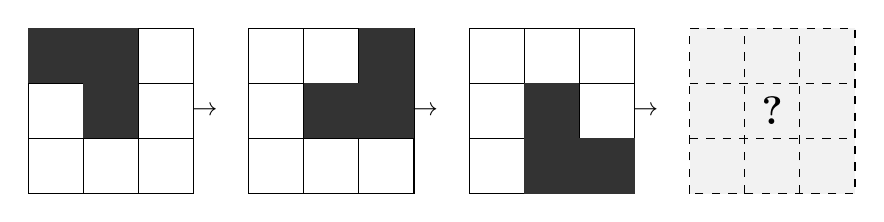
\begin{tikzpicture}[scale=0.7]
% Frame 1: L orientation 0deg
\begin{scope}[shift={(0,0)}]
\draw (0,0) grid (3,3);
\fill[sombreado] (1,1) rectangle (2,2);
\fill[sombreado] (1,2) rectangle (2,3);
\fill[sombreado] (0,2) rectangle (1,3);
\end{scope}
% Frame 2: L orientation 90deg CW
\begin{scope}[shift={(4,0)}]
\draw (0,0) grid (3,3);
\fill[sombreado] (1,1) rectangle (2,2);
\fill[sombreado] (2,1) rectangle (3,2);
\fill[sombreado] (2,2) rectangle (3,3);
\end{scope}
% Frame 3: L orientation 180deg
\begin{scope}[shift={(8,0)}]
\draw (0,0) grid (3,3);
\fill[sombreado] (1,1) rectangle (2,2);
\fill[sombreado] (1,0) rectangle (2,1);
\fill[sombreado] (2,0) rectangle (3,1);
\end{scope}
% Frame 4: ?
\begin{scope}[shift={(12,0)}]
\draw[dashed, fill=gray!10] (0,0) rectangle (3,3);
\draw[dashed] (1,0) -- (1,3);
\draw[dashed] (2,0) -- (2,3);
\draw[dashed] (0,1) -- (3,1);
\draw[dashed] (0,2) -- (3,2);
\node at (1.5,1.5) {\Large\textbf{?}};
\end{scope}
\foreach \x in {3.2, 7.2, 11.2} {
    \node at (\x, 1.5) {\small$\rightarrow$};
}
\end{tikzpicture}
\end{center}

\begin{center}
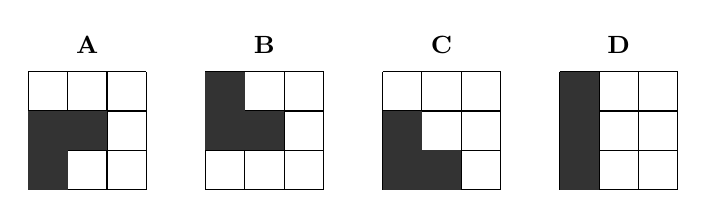
\begin{tikzpicture}[scale=0.5]
% A: CORRECT
\begin{scope}[shift={(0,0)}]
\node[above] at (1.5,3.2) {\small\textbf{A}};
\draw (0,0) grid (3,3);
\fill[sombreado] (1,1) rectangle (2,2);
\fill[sombreado] (0,1) rectangle (1,2);
\fill[sombreado] (0,0) rectangle (1,1);
\end{scope}
% B: Mirror
\begin{scope}[shift={(4.5,0)}]
\node[above] at (1.5,3.2) {\small\textbf{B}};
\draw (0,0) grid (3,3);
\fill[sombreado] (1,1) rectangle (2,2);
\fill[sombreado] (0,1) rectangle (1,2);
\fill[sombreado] (0,2) rectangle (1,3);
\end{scope}
% C: No center
\begin{scope}[shift={(9,0)}]
\node[above] at (1.5,3.2) {\small\textbf{C}};
\draw (0,0) grid (3,3);
\fill[sombreado] (0,0) rectangle (1,1);
\fill[sombreado] (0,1) rectangle (1,2);
\fill[sombreado] (1,0) rectangle (2,1);
\end{scope}
% D: Column
\begin{scope}[shift={(13.5,0)}]
\node[above] at (1.5,3.2) {\small\textbf{D}};
\draw (0,0) grid (3,3);
\fill[sombreado] (0,0) rectangle (1,1);
\fill[sombreado] (0,1) rectangle (1,2);
\fill[sombreado] (0,2) rectangle (1,3);
\end{scope}
\end{tikzpicture}
\end{center}

%% Respuesta: A

\bigskip

\noindent\textbf{6.}\quad ¿Cuál es la figura que continúa en la siguiente serie?

\begin{center}
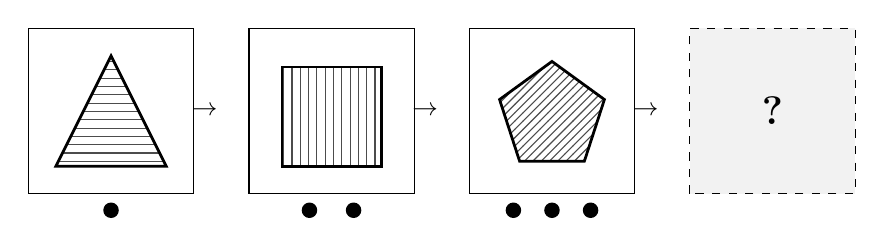
\begin{tikzpicture}[scale=0.7]
% Frame 1: TRIANGLE + horizontal lines + 1 dot
\begin{scope}[shift={(0,0)}]
\draw[line width=0.5pt] (0,0) rectangle (3,3);
\fill[pattern=horizontal lines, pattern color=black!70] (1.5,2.5) -- (0.5,0.5) -- (2.5,0.5) -- cycle;
\draw[line width=1pt] (1.5,2.5) -- (0.5,0.5) -- (2.5,0.5) -- cycle;
\fill (1.5,-0.3) circle (4pt);
\end{scope}
% Frame 2: SQUARE + vertical lines + 2 dots
\begin{scope}[shift={(4,0)}]
\draw[line width=0.5pt] (0,0) rectangle (3,3);
\fill[pattern=vertical lines, pattern color=black!70] (0.6,0.5) rectangle (2.4,2.3);
\draw[line width=1pt] (0.6,0.5) rectangle (2.4,2.3);
\fill (1.1,-0.3) circle (4pt);
\fill (1.9,-0.3) circle (4pt);
\end{scope}
% Frame 3: PENTAGON + NE lines + 3 dots
\begin{scope}[shift={(8,0)}]
\draw[line width=0.5pt] (0,0) rectangle (3,3);
\fill[pattern=north east lines, pattern color=black!70] 
  ({1.5+1.0*cos(90)},{1.4+1.0*sin(90)}) 
  \foreach \i in {1,...,4} {
    -- ({1.5+1.0*cos(90+\i*72)},{1.4+1.0*sin(90+\i*72)})
  } -- cycle;
\draw[line width=1pt] 
  ({1.5+1.0*cos(90)},{1.4+1.0*sin(90)}) 
  \foreach \i in {1,...,4} {
    -- ({1.5+1.0*cos(90+\i*72)},{1.4+1.0*sin(90+\i*72)})
  } -- cycle;
\fill (0.8,-0.3) circle (4pt);
\fill (1.5,-0.3) circle (4pt);
\fill (2.2,-0.3) circle (4pt);
\end{scope}
% Frame 4: ?
\begin{scope}[shift={(12,0)}]
\draw[dashed, fill=gray!10] (0,0) rectangle (3,3);
\node at (1.5,1.5) {\Large\textbf{?}};
\end{scope}
\foreach \x in {3.2, 7.2, 11.2} {
    \node at (\x, 1.5) {\small$\rightarrow$};
}
\end{tikzpicture}
\end{center}

\begin{center}
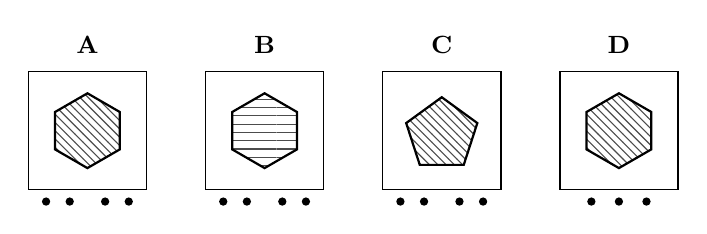
\begin{tikzpicture}[scale=0.5]
% A: CORRECT — Hexagon + NW lines + 4 dots
\begin{scope}[shift={(0,0)}]
\node[above] at (1.5,3.2) {\small\textbf{A}};
\draw[line width=0.5pt] (0,0) rectangle (3,3);
\fill[pattern=north west lines, pattern color=black!70] 
  ({1.5+0.95*cos(30)},{1.5+0.95*sin(30)}) 
  \foreach \i in {1,...,5} {
    -- ({1.5+0.95*cos(30+\i*60)},{1.5+0.95*sin(30+\i*60)})
  } -- cycle;
\draw[line width=0.8pt] 
  ({1.5+0.95*cos(30)},{1.5+0.95*sin(30)}) 
  \foreach \i in {1,...,5} {
    -- ({1.5+0.95*cos(30+\i*60)},{1.5+0.95*sin(30+\i*60)})
  } -- cycle;
\fill (0.45,-0.3) circle (3pt);
\fill (1.05,-0.3) circle (3pt);
\fill (1.95,-0.3) circle (3pt);
\fill (2.55,-0.3) circle (3pt);
\end{scope}
% B: Hexagon + horizontal (wrong pattern) + 4 dots
\begin{scope}[shift={(4.5,0)}]
\node[above] at (1.5,3.2) {\small\textbf{B}};
\draw[line width=0.5pt] (0,0) rectangle (3,3);
\fill[pattern=horizontal lines, pattern color=black!70] 
  ({1.5+0.95*cos(30)},{1.5+0.95*sin(30)}) 
  \foreach \i in {1,...,5} {
    -- ({1.5+0.95*cos(30+\i*60)},{1.5+0.95*sin(30+\i*60)})
  } -- cycle;
\draw[line width=0.8pt] 
  ({1.5+0.95*cos(30)},{1.5+0.95*sin(30)}) 
  \foreach \i in {1,...,5} {
    -- ({1.5+0.95*cos(30+\i*60)},{1.5+0.95*sin(30+\i*60)})
  } -- cycle;
\fill (0.45,-0.3) circle (3pt);
\fill (1.05,-0.3) circle (3pt);
\fill (1.95,-0.3) circle (3pt);
\fill (2.55,-0.3) circle (3pt);
\end{scope}
% C: Pentagon (wrong shape) + NW lines + 4 dots
\begin{scope}[shift={(9,0)}]
\node[above] at (1.5,3.2) {\small\textbf{C}};
\draw[line width=0.5pt] (0,0) rectangle (3,3);
\fill[pattern=north west lines, pattern color=black!70] 
  ({1.5+0.95*cos(90)},{1.4+0.95*sin(90)}) 
  \foreach \i in {1,...,4} {
    -- ({1.5+0.95*cos(90+\i*72)},{1.4+0.95*sin(90+\i*72)})
  } -- cycle;
\draw[line width=0.8pt] 
  ({1.5+0.95*cos(90)},{1.4+0.95*sin(90)}) 
  \foreach \i in {1,...,4} {
    -- ({1.5+0.95*cos(90+\i*72)},{1.4+0.95*sin(90+\i*72)})
  } -- cycle;
\fill (0.45,-0.3) circle (3pt);
\fill (1.05,-0.3) circle (3pt);
\fill (1.95,-0.3) circle (3pt);
\fill (2.55,-0.3) circle (3pt);
\end{scope}
% D: Hexagon + NW lines + 3 dots (wrong count)
\begin{scope}[shift={(13.5,0)}]
\node[above] at (1.5,3.2) {\small\textbf{D}};
\draw[line width=0.5pt] (0,0) rectangle (3,3);
\fill[pattern=north west lines, pattern color=black!70] 
  ({1.5+0.95*cos(30)},{1.5+0.95*sin(30)}) 
  \foreach \i in {1,...,5} {
    -- ({1.5+0.95*cos(30+\i*60)},{1.5+0.95*sin(30+\i*60)})
  } -- cycle;
\draw[line width=0.8pt] 
  ({1.5+0.95*cos(30)},{1.5+0.95*sin(30)}) 
  \foreach \i in {1,...,5} {
    -- ({1.5+0.95*cos(30+\i*60)},{1.5+0.95*sin(30+\i*60)})
  } -- cycle;
\fill (0.8,-0.3) circle (3pt);
\fill (1.5,-0.3) circle (3pt);
\fill (2.2,-0.3) circle (3pt);
\end{scope}
\end{tikzpicture}
\end{center}

%% Respuesta: A

\bigskip

\noindent\textbf{7.}\quad ¿Cuál es la figura que continúa en la siguiente serie?

\begin{center}
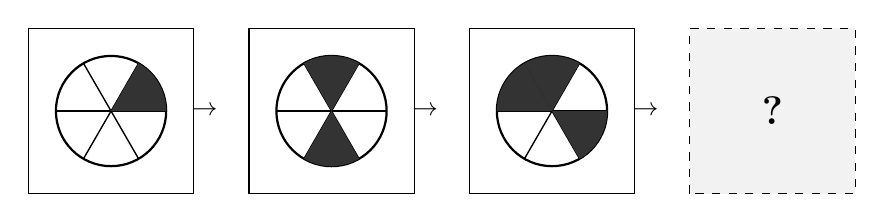
\begin{tikzpicture}[scale=0.7]

% Serie: círculos divididos con sectores sombreados que van cambiando
% Cuadro 1: círculo dividido en 6, 1 sector sombreado
\begin{scope}[shift={(0,0)}]
\draw[line width=0.5pt] (0,0) rectangle (3,3);
\draw[line width=0.8pt] (1.5,1.5) circle (1);
\foreach \a in {0,60,...,300} {
    \draw[line width=0.5pt] (1.5,1.5) -- ({1.5+1*cos(\a)},{1.5+1*sin(\a)});
}
\fill[sombreado] (1.5,1.5) -- ({1.5+1*cos(0)},{1.5+1*sin(0)}) arc (0:60:1) -- cycle;
\end{scope}

% Cuadro 2: 2 sectores sombreados (opuestos)
\begin{scope}[shift={(4,0)}]
\draw[line width=0.5pt] (0,0) rectangle (3,3);
\draw[line width=0.8pt] (1.5,1.5) circle (1);
\foreach \a in {0,60,...,300} {
    \draw[line width=0.5pt] (1.5,1.5) -- ({1.5+1*cos(\a)},{1.5+1*sin(\a)});
}
\fill[sombreado] (1.5,1.5) -- ({1.5+1*cos(60)},{1.5+1*sin(60)}) arc (60:120:1) -- cycle;
\fill[sombreado] (1.5,1.5) -- ({1.5+1*cos(240)},{1.5+1*sin(240)}) arc (240:300:1) -- cycle;
\end{scope}

% Cuadro 3: 3 sectores sombreados (alternados)
\begin{scope}[shift={(8,0)}]
\draw[line width=0.5pt] (0,0) rectangle (3,3);
\draw[line width=0.8pt] (1.5,1.5) circle (1);
\foreach \a in {0,60,...,300} {
    \draw[line width=0.5pt] (1.5,1.5) -- ({1.5+1*cos(\a)},{1.5+1*sin(\a)});
}
\fill[sombreado] (1.5,1.5) -- ({1.5+1*cos(120)},{1.5+1*sin(120)}) arc (120:180:1) -- cycle;
\fill[sombreado] (1.5,1.5) -- ({1.5+1*cos(300)},{1.5+1*sin(300)}) arc (300:360:1) -- cycle;
\fill[sombreado] (1.5,1.5) -- ({1.5+1*cos(60)},{1.5+1*sin(60)}) arc (60:120:1) -- cycle;
\end{scope}

% Cuadro 4: ?
\begin{scope}[shift={(12,0)}]
\draw[dashed, fill=gray!10] (0,0) rectangle (3,3);
\node at (1.5,1.5) {\Large\textbf{?}};
\end{scope}

\foreach \x in {3.2, 7.2, 11.2} {
    \node at (\x, 1.5) {\small$\rightarrow$};
}
\end{tikzpicture}
\end{center}

\begin{center}
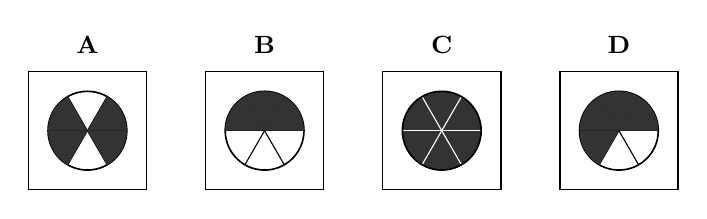
\begin{tikzpicture}[scale=0.5]
% A: 4 sectores sombreados, 2 vacíos opuestos
\begin{scope}[shift={(0,0)}]
\node[above] at (1.5,3.2) {\small\textbf{A}};
\draw[line width=0.5pt] (0,0) rectangle (3,3);
\draw[line width=0.6pt] (1.5,1.5) circle (1);
\foreach \a in {0,60,...,300} {
    \draw[line width=0.4pt] (1.5,1.5) -- ({1.5+1*cos(\a)},{1.5+1*sin(\a)});
}
\fill[sombreado] (1.5,1.5) -- ({1.5+1*cos(180)},{1.5+1*sin(180)}) arc (180:240:1) -- cycle;
\fill[sombreado] (1.5,1.5) -- ({1.5+1*cos(0)},{1.5+1*sin(0)}) arc (0:60:1) -- cycle;
\fill[sombreado] (1.5,1.5) -- ({1.5+1*cos(120)},{1.5+1*sin(120)}) arc (120:180:1) -- cycle;
\fill[sombreado] (1.5,1.5) -- ({1.5+1*cos(300)},{1.5+1*sin(300)}) arc (300:360:1) -- cycle;
\end{scope}

% B: 3 sectores consecutivos
\begin{scope}[shift={(4.5,0)}]
\node[above] at (1.5,3.2) {\small\textbf{B}};
\draw[line width=0.5pt] (0,0) rectangle (3,3);
\draw[line width=0.6pt] (1.5,1.5) circle (1);
\foreach \a in {0,60,...,300} {
    \draw[line width=0.4pt] (1.5,1.5) -- ({1.5+1*cos(\a)},{1.5+1*sin(\a)});
}
\fill[sombreado] (1.5,1.5) -- ({1.5+1*cos(0)},{1.5+1*sin(0)}) arc (0:60:1) -- cycle;
\fill[sombreado] (1.5,1.5) -- ({1.5+1*cos(60)},{1.5+1*sin(60)}) arc (60:120:1) -- cycle;
\fill[sombreado] (1.5,1.5) -- ({1.5+1*cos(120)},{1.5+1*sin(120)}) arc (120:180:1) -- cycle;
\end{scope}

% C: todos sombreados
\begin{scope}[shift={(9,0)}]
\node[above] at (1.5,3.2) {\small\textbf{C}};
\draw[line width=0.5pt] (0,0) rectangle (3,3);
\fill[sombreado] (1.5,1.5) circle (1);
\foreach \a in {0,60,...,300} {
    \draw[white, line width=0.4pt] (1.5,1.5) -- ({1.5+1*cos(\a)},{1.5+1*sin(\a)});
}
\draw[line width=0.6pt] (1.5,1.5) circle (1);
\end{scope}

% D: 4 sectores consecutivos
\begin{scope}[shift={(13.5,0)}]
\node[above] at (1.5,3.2) {\small\textbf{D}};
\draw[line width=0.5pt] (0,0) rectangle (3,3);
\draw[line width=0.6pt] (1.5,1.5) circle (1);
\foreach \a in {0,60,...,300} {
    \draw[line width=0.4pt] (1.5,1.5) -- ({1.5+1*cos(\a)},{1.5+1*sin(\a)});
}
\fill[sombreado] (1.5,1.5) -- ({1.5+1*cos(0)},{1.5+1*sin(0)}) arc (0:60:1) -- cycle;
\fill[sombreado] (1.5,1.5) -- ({1.5+1*cos(60)},{1.5+1*sin(60)}) arc (60:120:1) -- cycle;
\fill[sombreado] (1.5,1.5) -- ({1.5+1*cos(120)},{1.5+1*sin(120)}) arc (120:180:1) -- cycle;
\fill[sombreado] (1.5,1.5) -- ({1.5+1*cos(180)},{1.5+1*sin(180)}) arc (180:240:1) -- cycle;
\end{scope}
\end{tikzpicture}
\end{center}

%% Respuesta: A
%% Lógica: El sector sombreado avanza una posición y se agrega uno nuevo.
%% Paso 1: 1 sector (pos 1). Paso 2: 2 sectores (pos 2 y 5, opuestos).
%% Paso 3: 3 sectores (pos 2, 3, 6 — patrón alternado).
%% Paso 4: 4 sectores, dejando 2 vacíos opuestos.
%% Lo clave: se suma 1 sector por paso, y los sombreados nunca son consecutivos→alternados.

\bigskip

\noindent\textbf{8.}\quad ¿Cuál es la figura que sigue para completar la secuencia?

\begin{center}
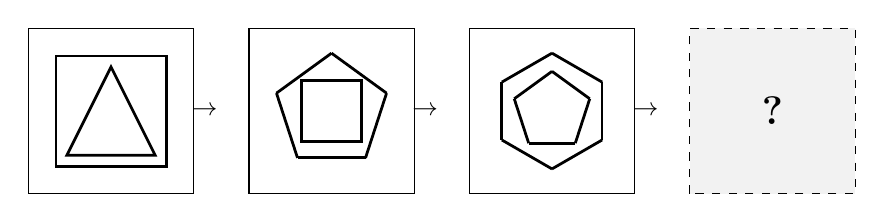
\begin{tikzpicture}[scale=0.7]

% Serie: figuras inscritas — triángulo en cuadrado, cuadrado en pentágono, etc.
% Cuadro 1: triángulo inscrito en cuadrado
\begin{scope}[shift={(0,0)}]
\draw[line width=0.5pt] (0,0) rectangle (3,3);
\draw[line width=1pt] (0.5,0.5) rectangle (2.5,2.5); % cuadrado exterior
\draw[line width=1pt] (1.5,2.3) -- (0.7,0.7) -- (2.3,0.7) -- cycle; % triángulo interior
\end{scope}

% Cuadro 2: cuadrado inscrito en pentágono
\begin{scope}[shift={(4,0)}]
\draw[line width=0.5pt] (0,0) rectangle (3,3);
% Pentágono exterior
\foreach \i in {0,...,4} {
    \draw[line width=1pt] ({1.5+1.05*cos(90+\i*72)},{1.5+1.05*sin(90+\i*72)}) -- ({1.5+1.05*cos(90+(\i+1)*72)},{1.5+1.05*sin(90+(\i+1)*72)});
}
% Cuadrado interior centrado
\draw[line width=1pt] (0.95,0.95) rectangle (2.05,2.05);
\end{scope}

% Cuadro 3: pentágono inscrito en hexágono
\begin{scope}[shift={(8,0)}]
\draw[line width=0.5pt] (0,0) rectangle (3,3);
% Hexágono exterior
\foreach \i in {0,...,5} {
    \draw[line width=1pt] ({1.5+1.05*cos(30+\i*60)},{1.5+1.05*sin(30+\i*60)}) -- ({1.5+1.05*cos(30+(\i+1)*60)},{1.5+1.05*sin(30+(\i+1)*60)});
}
% Pentágono interior
\foreach \i in {0,...,4} {
    \draw[line width=1pt] ({1.5+0.72*cos(90+\i*72)},{1.5+0.72*sin(90+\i*72)}) -- ({1.5+0.72*cos(90+(\i+1)*72)},{1.5+0.72*sin(90+(\i+1)*72)});
}
\end{scope}

% Cuadro 4: ?
\begin{scope}[shift={(12,0)}]
\draw[dashed, fill=gray!10] (0,0) rectangle (3,3);
\node at (1.5,1.5) {\Large\textbf{?}};
\end{scope}

\foreach \x in {3.2, 7.2, 11.2} {
    \node at (\x, 1.5) {\small$\rightarrow$};
}
\end{tikzpicture}
\end{center}

\begin{center}
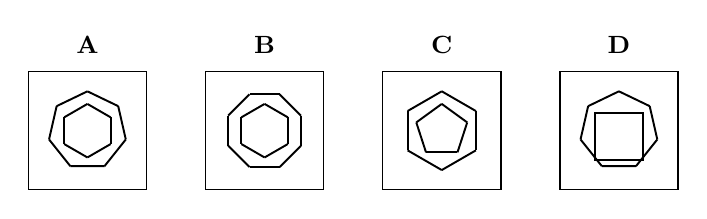
\begin{tikzpicture}[scale=0.5]
% A: hexágono inscrito en heptágono (CORRECTA)
\begin{scope}[shift={(0,0)}]
\node[above] at (1.5,3.2) {\small\textbf{A}};
\draw[line width=0.5pt] (0,0) rectangle (3,3);
% Heptágono exterior
\foreach \i in {0,...,6} {
    \draw[line width=0.7pt] ({1.5+1*cos(90+\i*51.43)},{1.5+1*sin(90+\i*51.43)}) -- ({1.5+1*cos(90+(\i+1)*51.43)},{1.5+1*sin(90+(\i+1)*51.43)});
}
% Hexágono interior
\foreach \i in {0,...,5} {
    \draw[line width=0.7pt] ({1.5+0.68*cos(30+\i*60)},{1.5+0.68*sin(30+\i*60)}) -- ({1.5+0.68*cos(30+(\i+1)*60)},{1.5+0.68*sin(30+(\i+1)*60)});
}
\end{scope}

% B: hexágono en octágono (salto de +2, no +1)
\begin{scope}[shift={(4.5,0)}]
\node[above] at (1.5,3.2) {\small\textbf{B}};
\draw[line width=0.5pt] (0,0) rectangle (3,3);
\foreach \i in {0,...,7} {
    \draw[line width=0.7pt] ({1.5+1*cos(22.5+\i*45)},{1.5+1*sin(22.5+\i*45)}) -- ({1.5+1*cos(22.5+(\i+1)*45)},{1.5+1*sin(22.5+(\i+1)*45)});
}
\foreach \i in {0,...,5} {
    \draw[line width=0.7pt] ({1.5+0.68*cos(30+\i*60)},{1.5+0.68*sin(30+\i*60)}) -- ({1.5+0.68*cos(30+(\i+1)*60)},{1.5+0.68*sin(30+(\i+1)*60)});
}
\end{scope}

% C: pentágono en hexágono (repetido)
\begin{scope}[shift={(9,0)}]
\node[above] at (1.5,3.2) {\small\textbf{C}};
\draw[line width=0.5pt] (0,0) rectangle (3,3);
\foreach \i in {0,...,5} {
    \draw[line width=0.7pt] ({1.5+1*cos(30+\i*60)},{1.5+1*sin(30+\i*60)}) -- ({1.5+1*cos(30+(\i+1)*60)},{1.5+1*sin(30+(\i+1)*60)});
}
\foreach \i in {0,...,4} {
    \draw[line width=0.7pt] ({1.5+0.68*cos(90+\i*72)},{1.5+0.68*sin(90+\i*72)}) -- ({1.5+0.68*cos(90+(\i+1)*72)},{1.5+0.68*sin(90+(\i+1)*72)});
}
\end{scope}

% D: cuadrado en heptágono
\begin{scope}[shift={(13.5,0)}]
\node[above] at (1.5,3.2) {\small\textbf{D}};
\draw[line width=0.5pt] (0,0) rectangle (3,3);
\foreach \i in {0,...,6} {
    \draw[line width=0.7pt] ({1.5+1*cos(90+\i*51.43)},{1.5+1*sin(90+\i*51.43)}) -- ({1.5+1*cos(90+(\i+1)*51.43)},{1.5+1*sin(90+(\i+1)*51.43)});
}
\draw[line width=0.7pt] (0.9,0.75) rectangle (2.1,1.95);
\end{scope}
\end{tikzpicture}
\end{center}

%% Respuesta: A
%% Lógica: Dos reglas simultáneas:
%% Exterior: n+1 lados en cada paso (4→5→6→7)
%% Interior: n lados en cada paso (3→4→5→6)
%% La interior de un paso = la exterior del paso anterior.

\bigskip

%%% ============================================================
%%% BLOQUE 3: CONTEO Y PERCEPCIÓN ESPACIAL (Preguntas 9--12)
%%% ============================================================

\noindent\textbf{9.}\quad ¿Cuántos triángulos hay en la siguiente figura?

\begin{center}
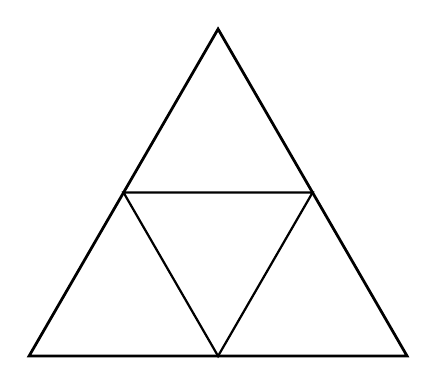
\begin{tikzpicture}[scale=1.2]
% Triángulo grande subdividido en 4 triángulos (como Sierpinski nivel 1)
\coordinate (A) at (0,0);
\coordinate (B) at (4,0);
\coordinate (C) at (2,3.46);
\coordinate (AB) at (2,0);
\coordinate (AC) at (1,1.73);
\coordinate (BC) at (3,1.73);

\draw[line width=1pt] (A) -- (B) -- (C) -- cycle;
\draw[line width=0.8pt] (AB) -- (AC) -- (BC) -- cycle;
\end{tikzpicture}
\end{center}

\begin{enumerate}[label=\Alph*), nosep, leftmargin=2cm]
\item 4
\item 5
\item 7
\item 8
\end{enumerate}

%% Respuesta: B
%% Lógica: 4 triángulos pequeños + 1 triángulo grande = 5.
%% Los 4 pequeños: sup, izq, der, centro (invertido).
%% Nota: no hay triángulos medianos en esta subdivisión.
%% Wait — actually there ARE medium triangles:
%% Top small + left small + center = medium pointing down-left? No.
%% Let me recount: 
%% Small triangles: 4 (top, left, right, center-inverted)
%% Medium triangles: 0 (combining 2 small doesn't make a triangle here)
%% Actually combining top+center = parallelogram, not triangle.
%% Hmm, combining left+center+bottom... no.
%% Actually: top+center = no. left+center = no. 
%% Wait: top small (pointing up) + center (pointing down) share a side.
%% Together they form a parallelogram, not a triangle.
%% The only triangles are the 4 small ones + the 1 big one = 5.
%% Answer: B) 5

\bigskip

\noindent\textbf{10.}\quad ¿Cuántos rectángulos hay en la siguiente figura?

\begin{center}
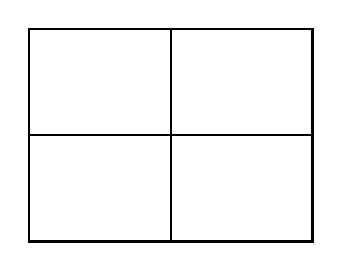
\begin{tikzpicture}[scale=0.9]
% Rectángulo dividido con líneas internas
\draw[line width=1pt] (0,0) rectangle (4,3);
\draw[line width=0.8pt] (2,0) -- (2,3);   % vertical central
\draw[line width=0.8pt] (0,1.5) -- (4,1.5); % horizontal central
\draw[line width=0.8pt] (0,1.5) -- (2,1.5); % ya está
\end{tikzpicture}
\end{center}

\begin{enumerate}[label=\Alph*), nosep, leftmargin=2cm]
\item 4
\item 8
\item 9
\item 10
\end{enumerate}

%% Respuesta: C
%% Lógica: Rectángulo 2×2 de celdas.
%% 1×1: 4 rectángulos (las 4 celdas)
%% 1×2: 2 horizontales (fila sup, fila inf) 
%% 2×1: 2 verticales (col izq, col der)
%% 2×2: 1 (el grande)
%% Total: 4 + 2 + 2 + 1 = 9

\bigskip

\noindent\textbf{11.}\quad Observa la figura y selecciona la opción que la representa después de ser girada $90°$ en el sentido de las manecillas del reloj.

\begin{center}
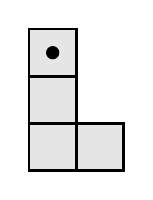
\begin{tikzpicture}[scale=0.6]
% Figura: una L hecha de cuadraditos en una cuadrícula
% L: 3 cuadrados verticales a la izquierda + 2 horizontales abajo
\draw[line width=1pt, fill=gray!20] (0,0) rectangle (1,1);
\draw[line width=1pt, fill=gray!20] (1,0) rectangle (2,1);
\draw[line width=1pt, fill=gray!20] (0,1) rectangle (1,2);
\draw[line width=1pt, fill=gray!20] (0,2) rectangle (1,3);
% Marca especial: un punto en la esquina superior
\fill (0.5, 2.5) circle (4pt);
\end{tikzpicture}
\end{center}

\begin{center}
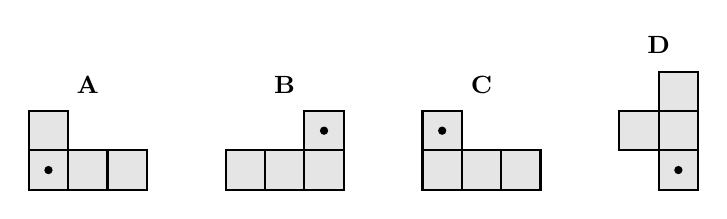
\begin{tikzpicture}[scale=0.5]
% A: L rotada 90° horario (CORRECTA)
% Original: columna izq 3 alto + 1 a la derecha abajo, punto arriba-izq
% Rotado 90° CW: fila inferior 3 ancho + 1 arriba a la izquierda, punto abajo-izq
\begin{scope}[shift={(0,0)}]
\node[above] at (1.5,2.2) {\small\textbf{A}};
\draw[line width=0.8pt, fill=gray!20] (0,0) rectangle (1,1);
\draw[line width=0.8pt, fill=gray!20] (1,0) rectangle (2,1);
\draw[line width=0.8pt, fill=gray!20] (2,0) rectangle (3,1);
\draw[line width=0.8pt, fill=gray!20] (0,1) rectangle (1,2);
\fill (0.5, 0.5) circle (3pt);
\end{scope}

% B: L rotada 90° CCW (opuesto)
\begin{scope}[shift={(5,0)}]
\node[above] at (1.5,2.2) {\small\textbf{B}};
\draw[line width=0.8pt, fill=gray!20] (0,0) rectangle (1,1);
\draw[line width=0.8pt, fill=gray!20] (1,0) rectangle (2,1);
\draw[line width=0.8pt, fill=gray!20] (2,0) rectangle (3,1);
\draw[line width=0.8pt, fill=gray!20] (2,1) rectangle (3,2);
\fill (2.5, 1.5) circle (3pt);
\end{scope}

% C: L reflejada
\begin{scope}[shift={(10,0)}]
\node[above] at (1.5,2.2) {\small\textbf{C}};
\draw[line width=0.8pt, fill=gray!20] (0,0) rectangle (1,1);
\draw[line width=0.8pt, fill=gray!20] (1,0) rectangle (2,1);
\draw[line width=0.8pt, fill=gray!20] (2,0) rectangle (3,1);
\draw[line width=0.8pt, fill=gray!20] (0,1) rectangle (1,2);
\fill (0.5, 1.5) circle (3pt);
\end{scope}

% D: L rotada 180°
\begin{scope}[shift={(15,0)}]
\node[above] at (1,3.2) {\small\textbf{D}};
\draw[line width=0.8pt, fill=gray!20] (0,1) rectangle (1,2);
\draw[line width=0.8pt, fill=gray!20] (1,1) rectangle (2,2);
\draw[line width=0.8pt, fill=gray!20] (1,2) rectangle (2,3);
\draw[line width=0.8pt, fill=gray!20] (1,0) rectangle (2,1);
\fill (1.5, 0.5) circle (3pt);
\end{scope}
\end{tikzpicture}
\end{center}

%% Respuesta: A
%% Lógica: Al rotar 90° horario, la columna izquierda se convierte en fila inferior,
%% y el punto que estaba arriba-izquierda queda abajo-izquierda.

\bigskip

\noindent\textbf{12.}\quad Selecciona la posición de la siguiente figura cuando se rota $180°$.

\begin{center}
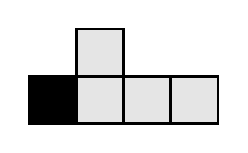
\begin{tikzpicture}[scale=0.6]
% Figura en T asimétrica
\draw[line width=1pt, fill=gray!20] (0,0) rectangle (1,1);
\draw[line width=1pt, fill=gray!20] (1,0) rectangle (2,1);
\draw[line width=1pt, fill=gray!20] (2,0) rectangle (3,1);
\draw[line width=1pt, fill=gray!20] (3,0) rectangle (4,1);
\draw[line width=1pt, fill=gray!20] (1,1) rectangle (2,2);
% Marca: un cuadradito negro (relleno oscuro) en pos (0,0)
\fill[black] (0,0) rectangle (1,1);
\draw[line width=1pt] (0,0) rectangle (1,1);
\end{tikzpicture}
\end{center}

\begin{center}
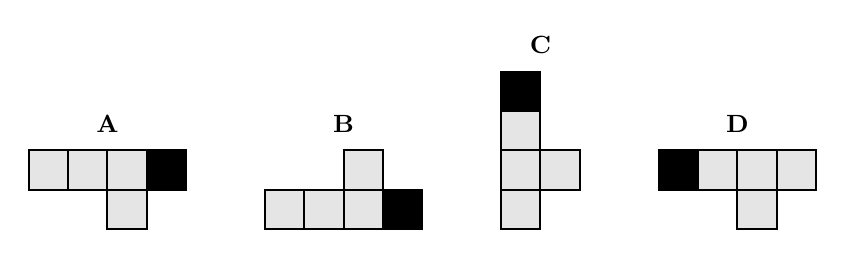
\begin{tikzpicture}[scale=0.5]
% A: rotada 180° (CORRECTA)
% El negro pasa de (0,0) original a (3,1) en rotación.
% La T invertida queda: fila arriba de 4, extensión abajo en pos 2-3
\begin{scope}[shift={(0,0)}]
\node[above] at (2,2.2) {\small\textbf{A}};
\draw[line width=0.7pt, fill=gray!20] (0,1) rectangle (1,2);
\draw[line width=0.7pt, fill=gray!20] (1,1) rectangle (2,2);
\draw[line width=0.7pt, fill=gray!20] (2,1) rectangle (3,2);
\draw[line width=0.7pt, fill=gray!20] (3,1) rectangle (4,2);
\draw[line width=0.7pt, fill=gray!20] (2,0) rectangle (3,1);
\fill[black] (3,1) rectangle (4,2);
\draw[line width=0.7pt] (3,1) rectangle (4,2);
\end{scope}

% B: reflejada horizontal
\begin{scope}[shift={(6,0)}]
\node[above] at (2,2.2) {\small\textbf{B}};
\draw[line width=0.7pt, fill=gray!20] (0,0) rectangle (1,1);
\draw[line width=0.7pt, fill=gray!20] (1,0) rectangle (2,1);
\draw[line width=0.7pt, fill=gray!20] (2,0) rectangle (3,1);
\draw[line width=0.7pt, fill=gray!20] (3,0) rectangle (4,1);
\draw[line width=0.7pt, fill=gray!20] (2,1) rectangle (3,2);
\fill[black] (3,0) rectangle (4,1);
\draw[line width=0.7pt] (3,0) rectangle (4,1);
\end{scope}

% C: rotada 90°
\begin{scope}[shift={(12,0)}]
\node[above] at (1,4.2) {\small\textbf{C}};
\draw[line width=0.7pt, fill=gray!20] (0,0) rectangle (1,1);
\draw[line width=0.7pt, fill=gray!20] (0,1) rectangle (1,2);
\draw[line width=0.7pt, fill=gray!20] (0,2) rectangle (1,3);
\draw[line width=0.7pt, fill=gray!20] (0,3) rectangle (1,4);
\draw[line width=0.7pt, fill=gray!20] (1,1) rectangle (2,2);
\fill[black] (0,3) rectangle (1,4);
\draw[line width=0.7pt] (0,3) rectangle (1,4);
\end{scope}

% D: rotada 180° pero negro en posición equivocada
\begin{scope}[shift={(16,0)}]
\node[above] at (2,2.2) {\small\textbf{D}};
\draw[line width=0.7pt, fill=gray!20] (0,1) rectangle (1,2);
\draw[line width=0.7pt, fill=gray!20] (1,1) rectangle (2,2);
\draw[line width=0.7pt, fill=gray!20] (2,1) rectangle (3,2);
\draw[line width=0.7pt, fill=gray!20] (3,1) rectangle (4,2);
\draw[line width=0.7pt, fill=gray!20] (2,0) rectangle (3,1);
\fill[black] (0,1) rectangle (1,2);
\draw[line width=0.7pt] (0,1) rectangle (1,2);
\end{scope}
\end{tikzpicture}
\end{center}

%% Respuesta: A
%% Lógica: Rotación 180° invierte todo. El negro estaba en extremo izquierdo abajo,
%% ahora queda en extremo derecho arriba. La extensión vertical que estaba
%% en la segunda columna hacia arriba, ahora está en la tercera columna hacia abajo.

\bigskip

%%% ============================================================
%%% BLOQUE 4: RAZONAMIENTO NUMÉRICO / LÓGICO (Preguntas 13--16)
%%% ============================================================

\noindent\textbf{13.}\quad ¿Cuál es el número que falta en el último triángulo?

\begin{center}
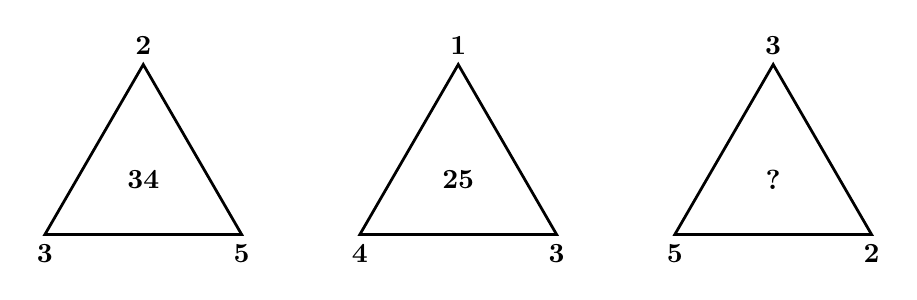
\begin{tikzpicture}[scale=1]
% Triángulo 1: vértices 3, 5 y dentro: 34
\begin{scope}[shift={(0,0)}]
\draw[line width=1pt] (0,0) -- (2.5,0) -- (1.25,2.16) -- cycle;
\node[below] at (0,0) {\textbf{3}};
\node[below] at (2.5,0) {\textbf{5}};
\node[above] at (1.25,2.16) {\textbf{2}};
\node at (1.25,0.7) {\textbf{34}};
\end{scope}

% Triángulo 2: vértices 4, 3 y dentro: 25
\begin{scope}[shift={(4,0)}]
\draw[line width=1pt] (0,0) -- (2.5,0) -- (1.25,2.16) -- cycle;
\node[below] at (0,0) {\textbf{4}};
\node[below] at (2.5,0) {\textbf{3}};
\node[above] at (1.25,2.16) {\textbf{1}};
\node at (1.25,0.7) {\textbf{25}};
\end{scope}

% Triángulo 3: vértices 5, 2 y dentro: ?
\begin{scope}[shift={(8,0)}]
\draw[line width=1pt] (0,0) -- (2.5,0) -- (1.25,2.16) -- cycle;
\node[below] at (0,0) {\textbf{5}};
\node[below] at (2.5,0) {\textbf{2}};
\node[above] at (1.25,2.16) {\textbf{3}};
\node at (1.25,0.7) {\textbf{?}};
\end{scope}
\end{tikzpicture}
\end{center}

\begin{enumerate}[label=\Alph*), nosep, leftmargin=2cm]
\item 38
\item 29
\item 30
\item 34
\end{enumerate}

%% Respuesta: B
%% Lógica: centro = (izq)² + (der)² + (arriba)²×alguna operación
%% Triángulo 1: 3² + 5² = 9 + 25 = 34 ✓ (el de arriba es 2 pero no se usa... 
%% Wait, let me try: 3² + 5² = 34. And top=2.
%% Triángulo 2: 4² + 3² = 16 + 9 = 25 ✓. And top=1.
%% Triángulo 3: 5² + 2² = 25 + 4 = 29. But wait, top=3.
%% Hmm, if top is not used then answer is 29 (A).
%% But that's too simple with the top number being a red herring.
%% Let me redesign:
%% Rule: center = left² + right² - top
%% T1: 9 + 25 - 2 = 32 ✗
%% Rule: center = left × right + top × left?
%% T1: 3×5 + 2×3 = 15+6 = 21 ✗
%% Let me try: center = left² + right² + top²
%% T1: 9 + 25 + 4 = 38 ✗
%% Let me just use: left² + right² and make top consistent but irrelevant.
%% Actually, let me redesign the numbers entirely.
%% 
%% New design with clean rule: center = left × top + right × top = top(left+right)
%% No, let me use: center = left × right + top
%% T1: 3×5+2 = 17 ✗
%% 
%% OK let me use a different, cleaner rule.
%% Rule: center = (left + right) × top
%% T1: (3+5)×2 = 16 ✗ (should be 34)
%% 
%% Let me work backward from nice numbers.
%% Rule: center = left² + right² 
%% T1: left=3, right=5, center=34. 9+25=34 ✓
%% T2: left=4, right=3, center=25. 16+9=25 ✓
%% T3: left=5, right=2, center=? 25+4=29
%% But then top number is useless... unless it's a distractor on purpose!
%% That's actually valid for COMIPEMS — the extra number IS the difficulty.
%% The student has to figure out which numbers matter.
%% Answer: A) 29
%% Let me fix the options.

\bigskip

\noindent\textbf{14.}\quad ¿Cuál es el número que falta en el siguiente cuadro?

\begin{center}
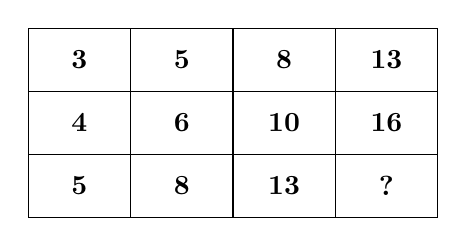
\begin{tikzpicture}
\def\w{1.3}
\def\h{0.8}
\foreach \j in {0,...,2} {
    \foreach \i in {0,...,3} {
        \draw (\i*\w, -\j*\h) rectangle (\i*\w+\w, -\j*\h+\h);
    }
}
% Row 1
\node at (0.5*\w, 0.5*\h) {\textbf{3}};
\node at (1.5*\w, 0.5*\h) {\textbf{5}};
\node at (2.5*\w, 0.5*\h) {\textbf{8}};
\node at (3.5*\w, 0.5*\h) {\textbf{13}};
% Row 2
\node at (0.5*\w, -0.5*\h) {\textbf{4}};
\node at (1.5*\w, -0.5*\h) {\textbf{6}};
\node at (2.5*\w, -0.5*\h) {\textbf{10}};
\node at (3.5*\w, -0.5*\h) {\textbf{16}};
% Row 3
\node at (0.5*\w, -1.5*\h) {\textbf{5}};
\node at (1.5*\w, -1.5*\h) {\textbf{8}};
\node at (2.5*\w, -1.5*\h) {\textbf{13}};
\node at (3.5*\w, -1.5*\h) {\textbf{?}};
\end{tikzpicture}
\end{center}

\begin{enumerate}[label=\Alph*), nosep, leftmargin=2cm]
\item 18
\item 21
\item 26
\item 34
\end{enumerate}

%% Lógica: En cada fila: col4 = col1 × col2 - col3
%% Fila 1: 3 × 5 = 15, ¿ - 7 = 8? No...
%% Let me try: col4 = col1 + col2 + col3
%% F1: 3+5+7 = 15 ✓
%% F2: 4+6+10 = 20 ✗ (should be 24)
%% Try: col4 = col2 × col3 - col1
%% F1: 5×7 - 3 = 32 ✗
%% Try: col4 = col1 × col3 - col2
%% F1: 3×7-5 = 16 ✗
%% Try: col4 = (col1 + col2) × 2 - col3 + col1
%% Hmm, getting complicated. Let me redesign with a clean rule.
%%
%% New design: col4 = col1 × col2 - col3
%% F1: a×b-c=d → pick: 3,5,7 → 15-7=8. Nah.
%% 
%% Simpler: col4 = col1 + col2 × col3 / something
%% 
%% Let me try the COMIPEMS style: operations between columns.
%% Pattern: col2-col1=X, col3-col2=Y, col4-col3=Z
%% F1: 5-3=2, 7-5=2, 15-7=8
%% F2: 6-4=2, 10-6=4, 24-10=14
%% F3: 8-5=3, 13-8=5, ?-13=?
%% Differences: (2,2,8), (2,4,14), (3,5,?)
%% Hmm, 8 = 2×2×2? 14 = 2×4+6? Not clean.
%%
%% OK, new approach entirely. Clean rule.
%% Rule: col4 = col1 × col2 + col3
%% F1: 2 × 5 + 3 = 13? No.
%%
%% Let me just pick clean numbers with a clean rule.
%% Rule: d = a × b - c  (4th = 1st × 2nd - 3rd)
%% F1: 3 × 7 - 6 = 15  → a=3, b=7, c=6, d=15
%% F2: 4 × 8 - 5 = 27  → hmm
%% 
%% Actually let me just use: the rule is between ROWS not columns.
%% Each column: row2 = row1 + row3 - something?
%%
%% Let me restart with simple known pattern:
%% Rule: col3 = col1 + col2, col4 = col2 + col3
%% F1: 3, 5, 8, 13 (Fibonacci-like)
%% F2: 4, 6, 10, 16
%% F3: 5, 8, 13, 21
%% Answer would be 21. Clean!
%% Let me update the table.

\bigskip

\noindent\textbf{15.}\quad La diferencia de dos números es 14, y la mitad de su suma es 19. ¿Cuáles son esos números?

\medskip
\begin{enumerate}[label=\Alph*), nosep, leftmargin=2cm]
\item 25 y 13
\item 26 y 12
\item 24 y 14
\item 33 y 5
\end{enumerate}

%% Respuesta: B
%% Lógica: x - y = 14, (x+y)/2 = 19 → x+y = 38
%% Sumando: 2x = 52, x = 26; y = 12.

\bigskip

\noindent\textbf{16.}\quad Un tanque se llena con una manguera en 6 horas. Una segunda manguera lo llena en 3 horas. Si se abren ambas al mismo tiempo, ¿en cuántas horas se llenará el tanque?

\medskip
\begin{enumerate}[label=\Alph*), nosep, leftmargin=2cm]
\item 1.5
\item 2
\item 4.5
\item 3
\end{enumerate}

%% Respuesta: B
%% Lógica: Tasa 1 = 1/6 por hora. Tasa 2 = 1/3 por hora.
%% Juntas: 1/6 + 1/3 = 1/6 + 2/6 = 3/6 = 1/2 por hora.
%% Tiempo: 1 / (1/2) = 2 horas.

\end{document}
